% Created 2018-10-25 Thu 19:12
% Intended LaTeX compiler: pdflatex
\documentclass[11pt]{article}
\usepackage[utf8]{inputenc}
\usepackage[T1]{fontenc}
\usepackage{graphicx}
\usepackage{grffile}
\usepackage{longtable}
\usepackage{wrapfig}
\usepackage{rotating}
\usepackage[normalem]{ulem}
\usepackage{amsmath}
\usepackage{textcomp}
\usepackage{amssymb}
\usepackage{capt-of}
\usepackage{hyperref}
\usepackage{color}
\usepackage{minted}
\usepackage{color}
\usepackage{minted}
\usepackage{parskip}
\usepackage{geometry}
\geometry{left=2.5cm,right=2.5cm,top=2.5cm,bottom=2.5cm}
\author{Daniel Moreno Manzano}
\date{\today}
\title{Quantum Volume}
\hypersetup{
 pdfauthor={Daniel Moreno Manzano},
 pdftitle={Quantum Volume},
 pdfkeywords={},
 pdfsubject={},
 pdfcreator={Emacs 25.1.1 (Org mode 9.0.5)}, 
 pdflang={English}}
\begin{document}

\maketitle


\section{Introduction}
\label{sec:org977cce4}

Given the different hardware implementations and technologies in Quantum Computation (superconducting, ion-trap, spin qubits, \ldots{}), it is often difficult to benchmark the usefulness or power of quantum systems. 
A \textbf{hardware-independent measure} is required to depict whether a device is able to run a quantum circuit or not.
Here is where the Quantum Volume metric appears on the scene.

The aim of Quantum Volume is to quantify the computational power of quantum devices. 
Consequently we will use it as a metric to measure the runnability of the quantum algorithms and the quantum devices -- \emph{\textbf{"can this algorithm be run in a given device?"}}.
While the device is the basis of the Quantum Volume metric, we fix our attention on the circuit.
Our purpose is to assert how the mapping procedure affects the runnability of a given circuit and to study how the Quantum Volume is related to the probability of success.

\section{Quantum Volume definition}
\label{sec:orgd65f145}

In this section, we define the Quantum Volume metric as well as the insights and ideas motivated by it.

\subsection{Literature review}
\label{sec:org1dd4c1a}

Few studies have been published on the Quantum Volume topic \cite{Bishop_2017,Moll_2018}.
In this section, a brief introduction to the metric is offered, reviewing the important concepts and basis.

\subsubsection{Hardware parameters}
\label{sec:org58baaf4}

The Quantum Volume metric considers that a quantum computer's performance mainly depends on the next hardware specifications:

\begin{itemize}
\item \(N\). The number of physical qubits
\item Quantum chip topology. The connectivity between qubits
\item Maximum number of sequential gates with correctable errors. The number of gates that can be applied before errors or decoherence mask the result
\item Gate set. Available hardware gate set
\item Maximum number of parallel operations. Number of operations that can be run in parallel
\end{itemize}

\subsubsection{Definitions and metrics}
\label{sec:org78619bb}

In this section we explain some required definitions, inferred from \cite{Bishop_2017,Moll_2018}, to understand Quantum Volume.


\begin{description}
\item[{Model algorithm.}] In the literature, Bishop uses the term \emph{model algorithm} \cite{Bishop_2017} to refer to a depth-one circuit, "constructed by random 2-qubit unitary matrix chosen uniformly over \(SU (4)\) on a random pairing of the qubits". Or, what is the same, the \emph{model algorithm} defines any single- or two-qubit gates combination as circuit unit. The mapping requirements of the device and the mapping quality is included as well. In the case that a two-qubit gate force any qubit to be routed, the gate additions will be included in the \emph{model algorithm}.
\end{description}

\begin{figure}[htbp]
\centering
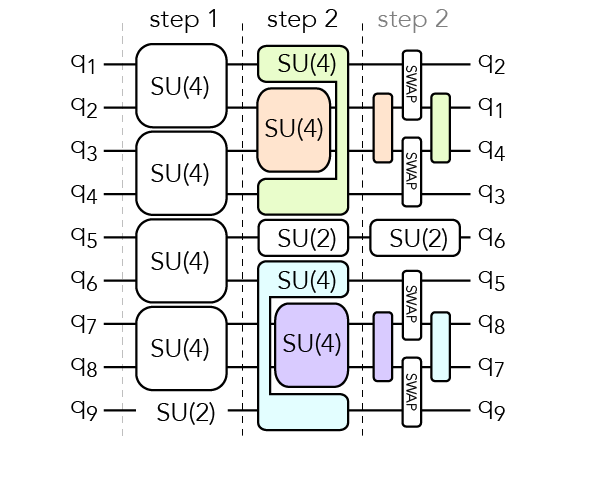
\includegraphics[width=0.7\textwidth]{model_algorithm.png}
\caption{\label{fig:org7953257}
Model algorithm example from \cite{Moll_2018}. Each step represents a possible combination of gates considered as \emph{model algorithm}. Notice that step 2 requires a mapping process that is shown afterwards.}
\end{figure}


\begin{description}
\item[{\(\textbf{n}\)}] Number of active qubits in a device of \(N\) qubits for a given algorithm.
\end{description}


\begin{description}
\item[{Effective error rate \(\epsilon_{eff} \approx 1/(d n)\).}] It is the error rate per \emph{model algorithm}, an averaged error over many realizations of depth-one circuits with random combinations of two-qubit gates. \(\epsilon_{eff}\) defines how well a device can implement arbitrary pairwise interactions between qubits. As soon as it is the error of the \emph{model algorithm}, it encapsulates errors of both single- and two-qubit gates. And it depends not only on the gate error rates and connectivity, but also on the sophistication of the scheduling algorithm responsible for mapping the model algorithm to the hardware.

\item[{Achievable circuit depth \(d(N) \simeq \frac{1}{N \epsilon_{eff}}\)}] Maximum circuit depth for which the results are correctable and useful in some device.
\end{description}

\begin{description}
\item[{Quantum Volume \(\tilde{V}_Q = min (N, d(N))^2\)}] quantifies the space-time volume occupied by a model circuit with random two-qubit gates that can be reliably executed on a given device.
\end{description}

\subsection{Insights and new ideas}
\label{sec:org9bba458}

After understading the concept of Quantum Volume, we derived some insights and we had ideas motivated by the possibilities that the new metric offers. 
We define \textbf{runnability} based on the separation of the concepts of \emph{device} Quantum Volume (\(V_Q\)) and \emph{algorithm} Quantum Volume (\(V^a_Q\)).

\subsubsection{Quantum Volume of a device}
\label{sec:org09a36bb}

Following \cite{Bishop_2017,Moll_2018}, we can expand the Quantum Volume general equation (\(\tilde{V}_Q\)) with the other definitions in the previous section and maximize for the biggest possible \(n\). 
Then, the maximum Quantum Volume that a device could run is defined by:

$$V_Q = \max_{n \le N} \min \left[ n,\frac{1}{n \epsilon_{eff} (n)}\right]^2$$

We define this Quantum Volume as the \emph{device} Quantum Volume. 
In Fig. \ref{fig:deviceQV2} and Fig. \ref{fig:deviceQV1} a graph describing the Quantum Volume as a function of \(n\) and \(\epsilon_{eff}\) is shown. 

%\begin{figure}

%\centering
\begin{minipage}{.45\textwidth}

\centering

\begin{center}
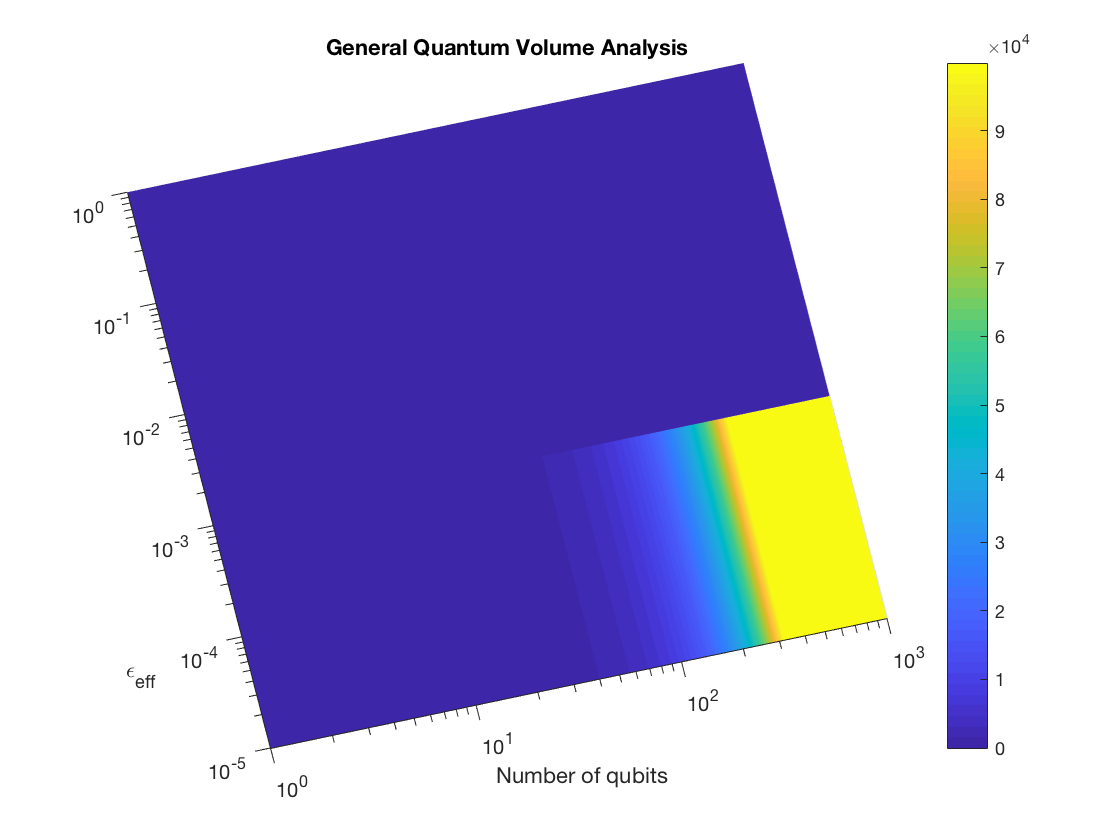
\includegraphics[width=.9\linewidth]{general_QV2.png}
\end{center}

\captionof{figure}{}
\label{fig:deviceQV2}

\end{minipage}%
\hspace{1cm}
\begin{minipage}{.45\textwidth}

\begin{center}
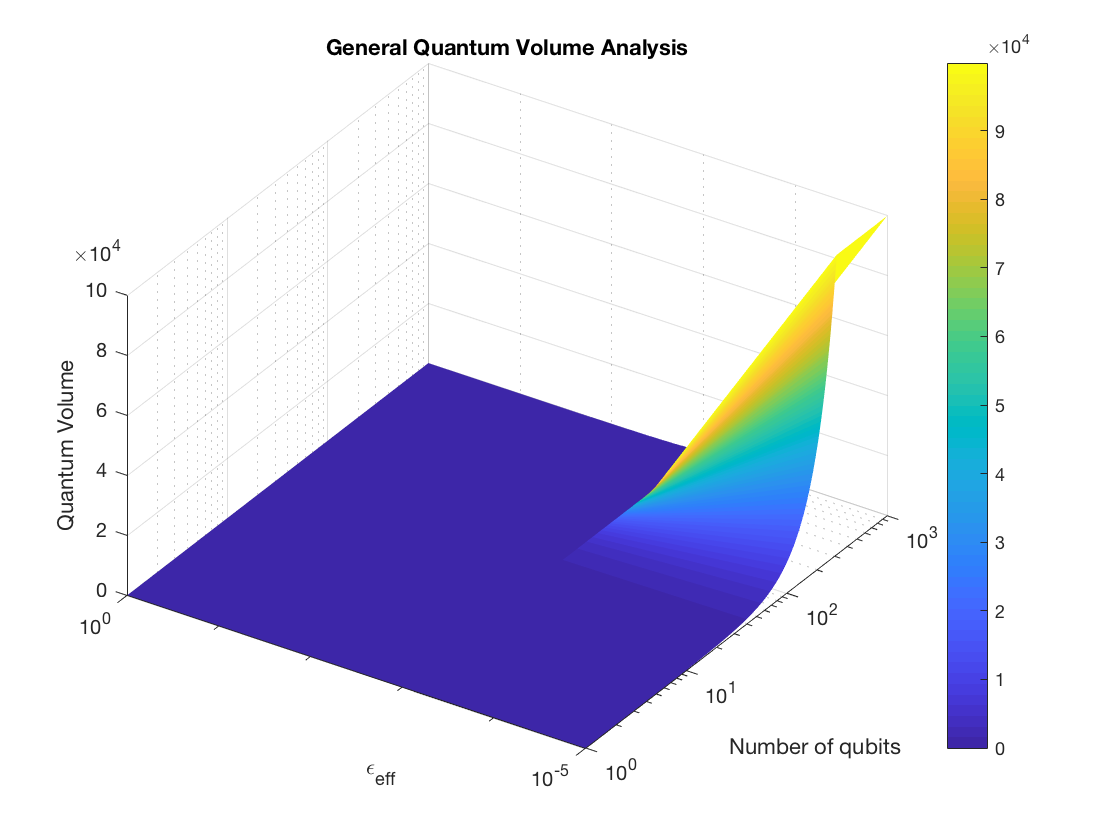
\includegraphics[width=.9\linewidth]{general_QV1.png}
\end{center}

\captionof{figure}{}
\label{fig:deviceQV1}

\end{minipage}%

\subsubsection{Quantum Volume of an algorithm}
\label{sec:orgf08f362}



$$V_Q^a = \min \left[ n,d \right]^2$$

%\begin{figure}

%\centering
\begin{minipage}{.45\textwidth}

\centering

\begin{center}
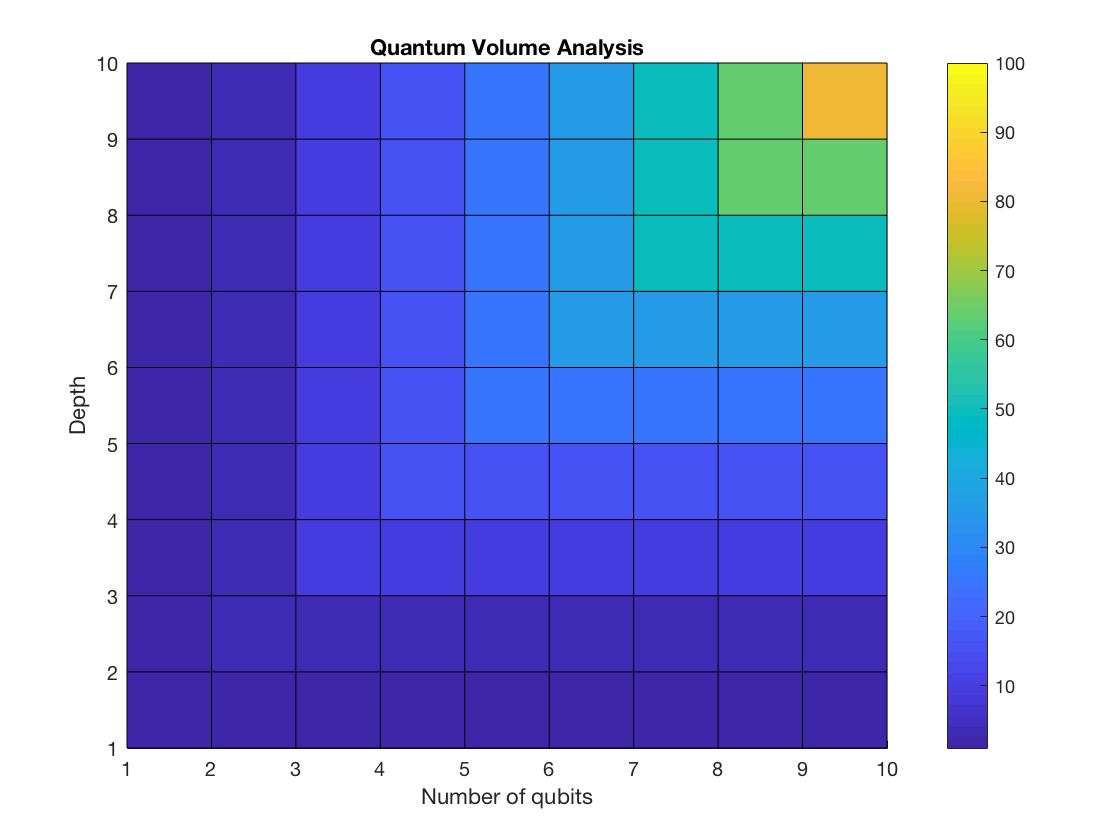
\includegraphics[width=.9\linewidth]{V_q_analysis2.png}
\end{center} 

\captionof{figure}{}
\label{fig:algorithmQV2}

\end{minipage}%
\hspace{1cm}
\begin{minipage}{.45\textwidth}

\begin{center}
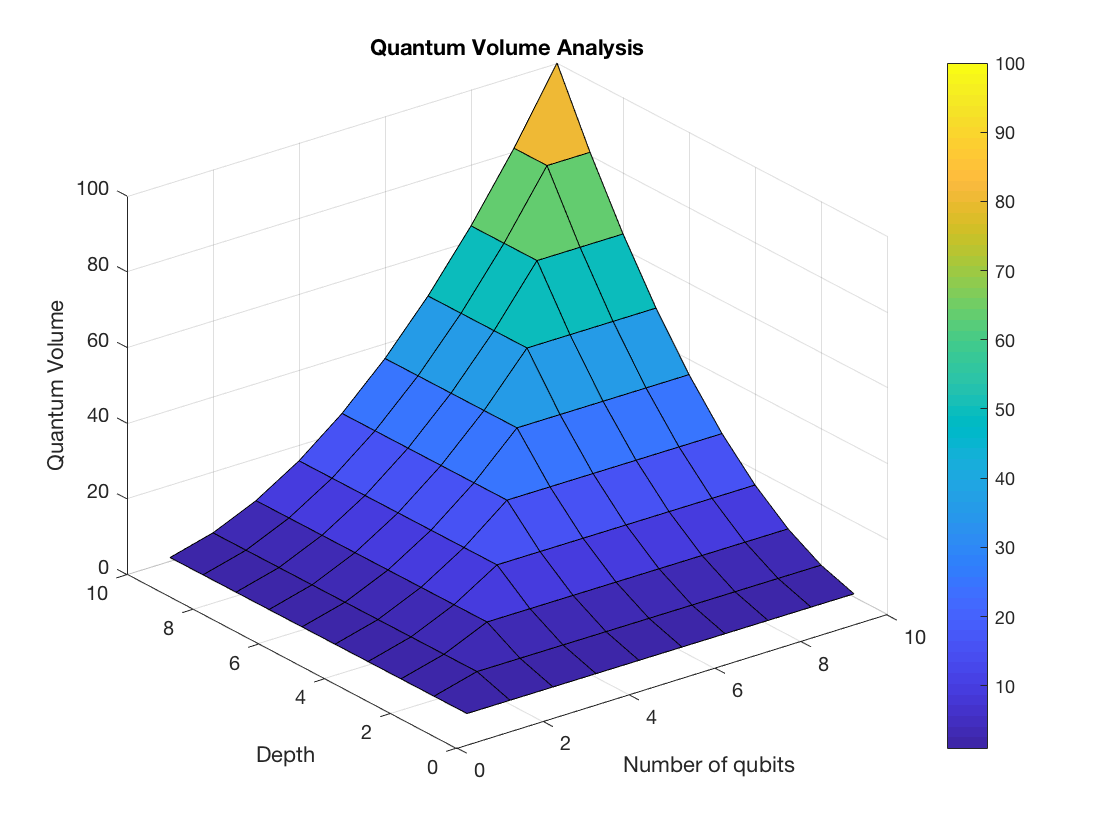
\includegraphics[width=.9\linewidth]{V_q_analysis1.png}
\end{center} 

\captionof{figure}{}
\label{fig:algorithmQV1}

\end{minipage}%

\subsubsection{Runnability}
\label{sec:org513bb98}

Following the \$\$

We define runnability as 

$$V_Q > V_Q^a$$

One may imagine the process of checking, whether or not, some cube with a given volume -- representing the algorithm -- would fit in a box -- the device --.

\section{Methodology}
\label{sec:org6467016}

\section{{\bfseries\sffamily TODO} Probability of success relation with Quantum Volume}
\label{sec:org65879e8}

\emph{How Quantum Volume is related with Probability of success?}

\emph{How to calculate \(\epsilon_{eff}\) with the methods of Probability of success?}



\section{BIB [delete this HEADER]}
\label{sec:org569c2b2}

\bibliography{../thesis_plan}
\bibliographystyle{plain}
\end{document}
